\section*{Introduction}\index{Polyneoptera}
Polyneoptera (Insecta: Pterygota: Neoptera) is a superordinal lineage, often with the rank of ``cohort'', that only recently has been shown to be monophyletic. Do you see characters that might represent synapomorphies? (Hint: there aren't many, unfortunately, but look at the hind wings.) Keep in mind that Plecoptera belongs in Polyneoptera but was treated earlier in order to focus on its aquatic biology and the origin of wings/flight.

\section{Dermaptera (earwigs)}\index{Dermaptera}
\begin{itemize}
\item body dorsoventrally flattened
\item head prognathous
\item fore wings relatively short, heavily sclerotized, elytraform
\item hind wing fan-shaped
\item cerci forceps-like, each cercus comprised of a single segment
\item defensive glands open near 3rd and 4th abdominal tergites
\end{itemize}
Several families occur in North America, but we'll cover two. A single diagnostic character is sufficient to separate these two in lab, but you should key \citep{engelDerm} your specimens out to confirm their identity. You could easily collect one of the families we \textit{don't} cover in lab.\vspace{3mm}

\begin{theo}
{}What do you think the sclerotized cerci are used for? Why are the fore wings so short, leaving so much abdomen exposed?
\end{theo} 

\subsubsection{Spongiphoridae (little earwigs; includes Labiidae)}\index{Spongiphoridae}
\noindent{}\textit{Diagnostic characters:} 2nd tarsomere cylindrical.\vspace{3mm}

\noindent{}\textit{Natural history:} About eight species occur in North America, and the common, invasive \textit{Labia minor} (Linnaeus, 1758) can be found at lights with relative ease.\vspace{3mm}

\begin{figure}[ht!]
  \centering
    \includegraphics[width=0.45\textwidth]{polyneoptera/spongiphoridae}
  \caption{\textit{Labia minor} (Spongiphoridae) \citep[modified from][Fig. 36; original by Mohr]{bhlitem105840ross}}
  \label{fig:spongi}
\end{figure}

\subsubsection{Forficulidae (European and spine-tailed earwigs)}\index{Forficulidae}
\noindent{}\textit{Diagnostic characters:} 2nd tarsomere lobed apically.\vspace{3mm}

\noindent{}\textit{Natural history:} This family is similar in habits and habitus to Spongiphoridae. Six species occur in he U.S., and they're all scavengers and opportunistic predators.\vspace{3mm}

\begin{figure}[ht!]
  \centering
    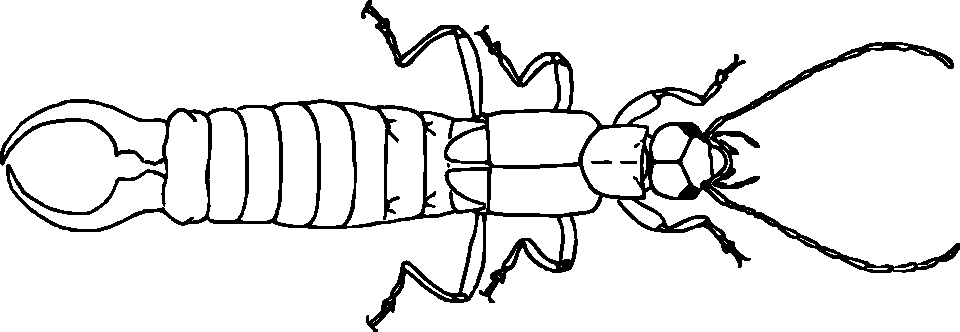
\includegraphics[width=0.65\textwidth]{polyneoptera/Forficulidae}
  \caption{Forficulidae \citep[Modified from][]{eisner1960defense}}
  \label{fig:forfic1}
\end{figure}

\section{Zoraptera}\index{Zoraptera}

\noindent{}Note that these insects are gregarious, and the overall phenotype of an individual depends on status of the aggregation.\vspace{3mm}

\noindent{}\textit{Diagnostic characters:} Pale, eyeless, wingless OR pigmented (brown), with small compound eyes and wings (wings are dehiscent though!); wings with relatively simple venation; tarsus with 2 tarsomeres; cerci comprised of one apparent segment (\textit{i.e.}, no subdivisions).\vspace{3mm}

\noindent{}\textit{Natural history:} There are two extant families---\textbf{Zorotypidae} and Spiralizoridae---with nearly 50 extant species worldwide. Zorapterans live in loose colonies in rotten wood (that must be \textit{just} right) and sawdust. Specimens are typically one of two forms: whitish, eyeless, wingless, and weakly sclerotized insects, or brownish, eyed, winged specimens (dispersal phase).\index{Zorotypidae}\vspace{3mm}

\begin{figure}[ht!]
    \centering
    \begin{subfigure}[ht!]{0.44\textwidth}
        \includegraphics[width=\textwidth]{polyneoptera/ZorotypidHabitus}
        \caption{}
        \label{fig:zorotypid1}
    \end{subfigure}
    \qquad
    \begin{subfigure}[ht!]{0.44\textwidth}
        \includegraphics[width=\textwidth]{polyneoptera/ZorotypidHabitus2}
        \caption{}
        \label{fig:zorotypid2}
    \end{subfigure}
    \caption{Zoraptera. (a) With eyes and wings \citep[][Figs. 1,5]{bhlpart32187}; (b) different forms \citep[][Figs. 2--4]{bhlpart32187}}\label{fig:zorotypids}
\end{figure}

\section{Orthoptera}\index{Orthoptera}
\begin{itemize}
\item head hypognathous
\item pronotum saddle-shaped
\item fore wing more sclerotized (tegmen) than hind wing
\item tarsus with 4 or fewer tarsomeres
\item hind leg saltatorial (femora enlarged)
\end{itemize}

\subsection{Caelifera (grasshoppers)}\index{Caelifera}
\begin{itemize}
\item antenna usually less than half as long as body, 
\item flagellum subdivided into less than 28 flagellomeres 
\item tarsi subdivided into 3 or fewer tarsomeres
\item auditory organ is absent from the foreleg and usually present on the first abdominal segment.
\item ovipositor short
\end{itemize}

\subsubsection{Tridactylidae (mole grasshoppers)}\index{Tridactylidae}% need to sight ID?
\noindent{}\textit{Diagnostic characters:} Pronotum does not extend over the length of the abdomen; fore and middle tarsi with 2 tarsomeres; fore wing reduced, stridulatory organ absent; hind tarsus absent or represented by one tarsomere, shorter than apical hind tibial spurs (Notice anything unusual about the phenotype of the hind leg?); body usually less than 20 mm long; auditory organ usually present on 1st abdominal segment.\vspace{3mm}

\noindent{}\textit{Natural history:} Less than 10 species live in the U.S. All of them can be found along the edges of aquatic habitats, \textit{e.g.}, in the sandy areas along a lake edge.\vspace{3mm}

\begin{theo}
{}Tridactylid hind legs are adapted for jumping off the surface of water. Can you see and interpret the structures that facilitate this amazing feat?
\end{theo} 

\begin{figure}[ht!]
  \centering
    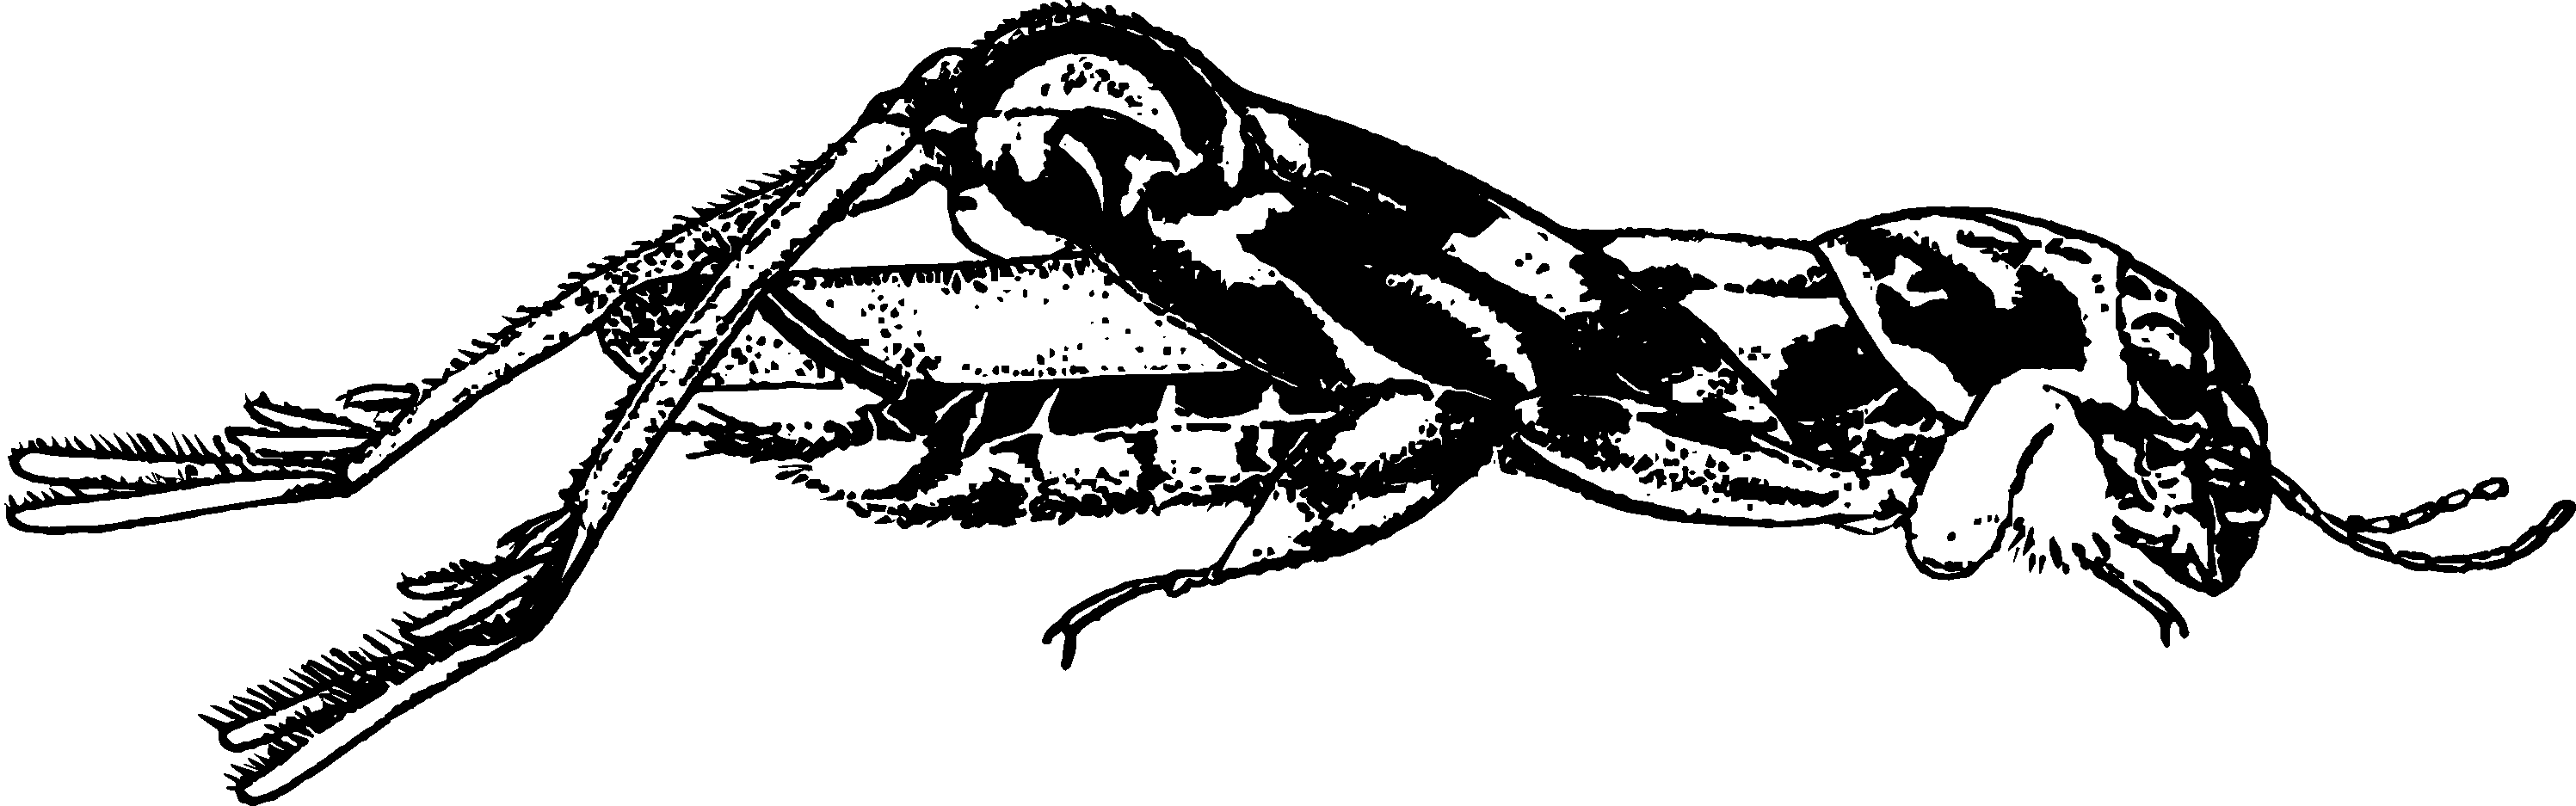
\includegraphics[width=0.7\textwidth]{polyneoptera/tridactylidae}
  \caption{Tridactylidae \citep[redrawn from][Fig. 5:1]{bhlitem126080aquatic}}
  \label{fig:tridact}
\end{figure}

\subsubsection{Tetrigidae (pygmy grasshoppers)}\index{Tetrigidae}
\noindent{}\textit{Diagnostic characters:} Pronotum extended posteriorly largely overlaps hind wing and extends over the length of abdomen; hind tarsus with more than one tarsomere (tarsal formula = 2-2-3); hind tarsus is longer than apical hind tibial spurs; body usually less than 20 mm long; fore wings are absent or vestigial; auditory organ absent.\vspace{3mm}

\noindent{}\textit{Natural history:} A diverse family worldwide ($\sim$1,600 described species), but only 30 or so occur in the U.S. They are closely associated with water usually.\vspace{3mm}

\begin{theo}
{}What is the function of the elongated pronotum? Is this structure perhaps taking over the function of another structure that is missing or reduced?
\end{theo}

\begin{figure}[ht!]
  \centering
     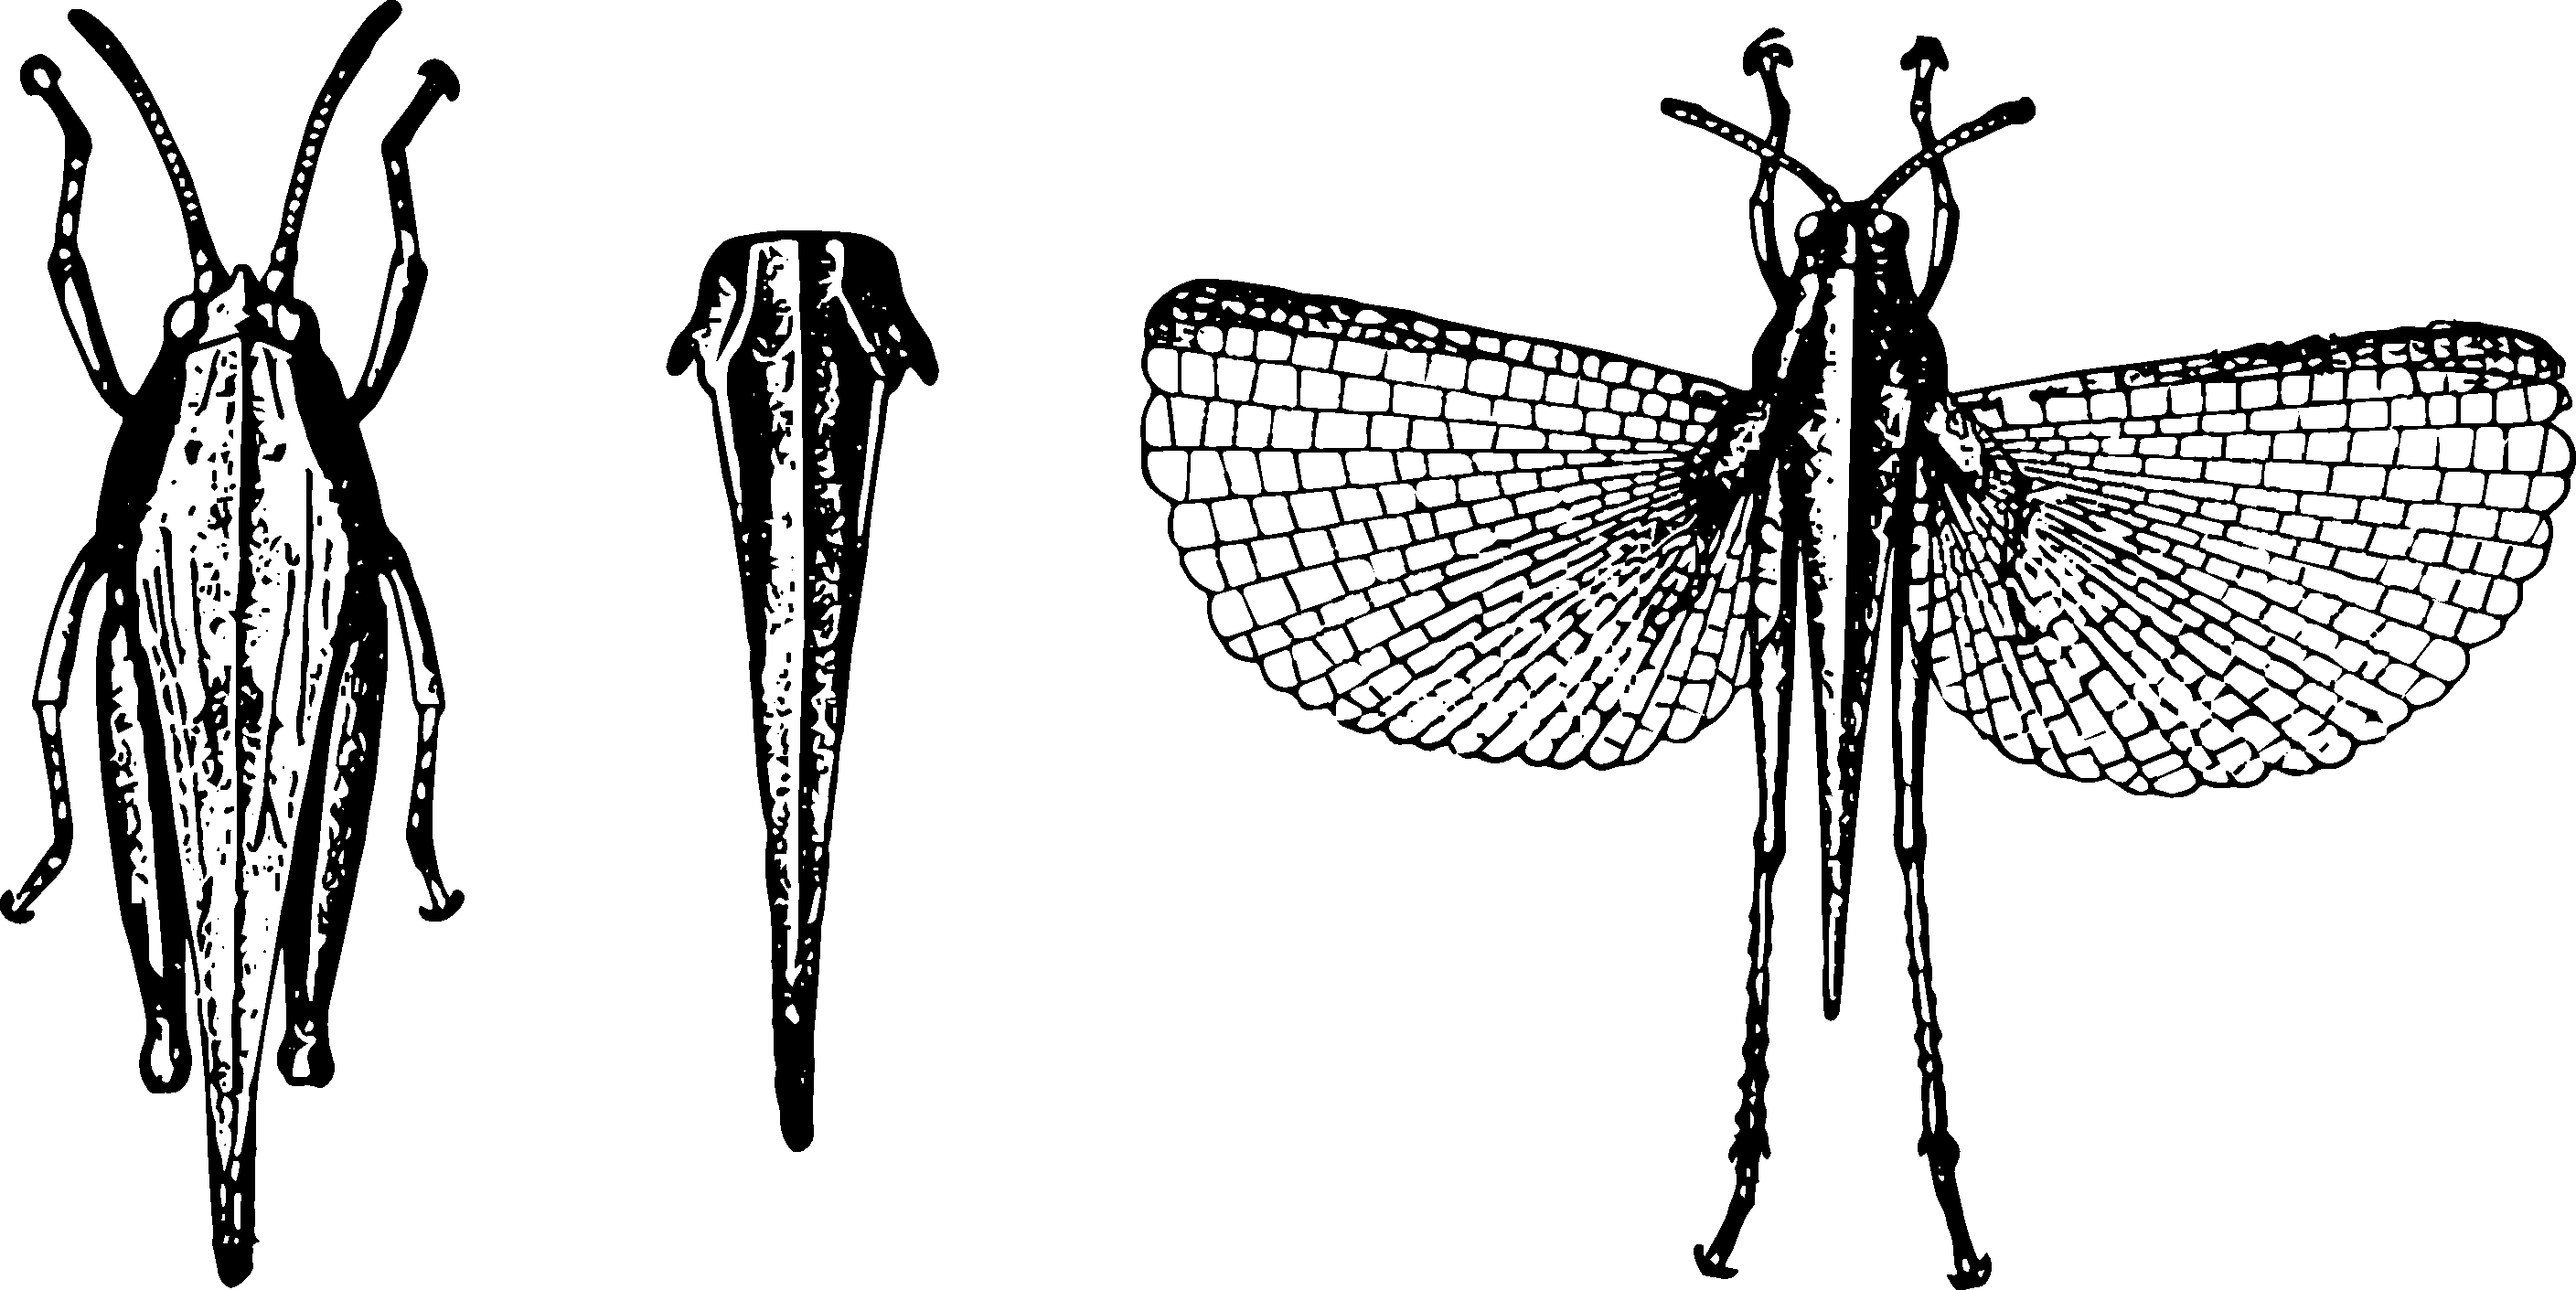
\includegraphics[width=0.75\textwidth]{polyneoptera/tetrigid}
  \caption{Tetrigidae \citep[modified from][Figs. 195--196]{kellogg1906american}}
  \label{fig:tetrig}
\end{figure}

\subsubsection{Acrididae (short-horned grasshoppers)}\index{Acrididae}
\noindent{}\textit{Diagnostic characters:} Pronotum not extended posteriorly, barely overlaps hind wing and does not extend over the length of the abdomen; fore wing well developed; hind tarsus with more than one tarsomere (each tarsus with 3 tarsomeres); hind tarsus is longer than apical hind tibial spurs; body usually more than 20 mm long; auditory organ usually present laterally on 1st abdominal segment.\vspace{3mm}

\noindent{}\textit{Natural history:} The most diverse family in Orthoptera, with $\sim$10,000 described species. Approximately 620 of these occur in the U.S., and they're all herbivores. Males stridulate.\vspace{3mm}

\noindent{}\textit{Specimen preparations:} Specimens should have at least one set of wings spread (right if possible), so that the color patterns can be visualized.\vspace{3mm}\index[preps]{Acrididae}%check field guide!!!

\begin{theo}
{}Grasshoppers have ears so that they can listen to each other. How do they make sounds? See figure \ref{fig:acrididhabitus} for a huge hint.
\end{theo}

\begin{figure}[ht!]
  \centering
    \reflectbox{
    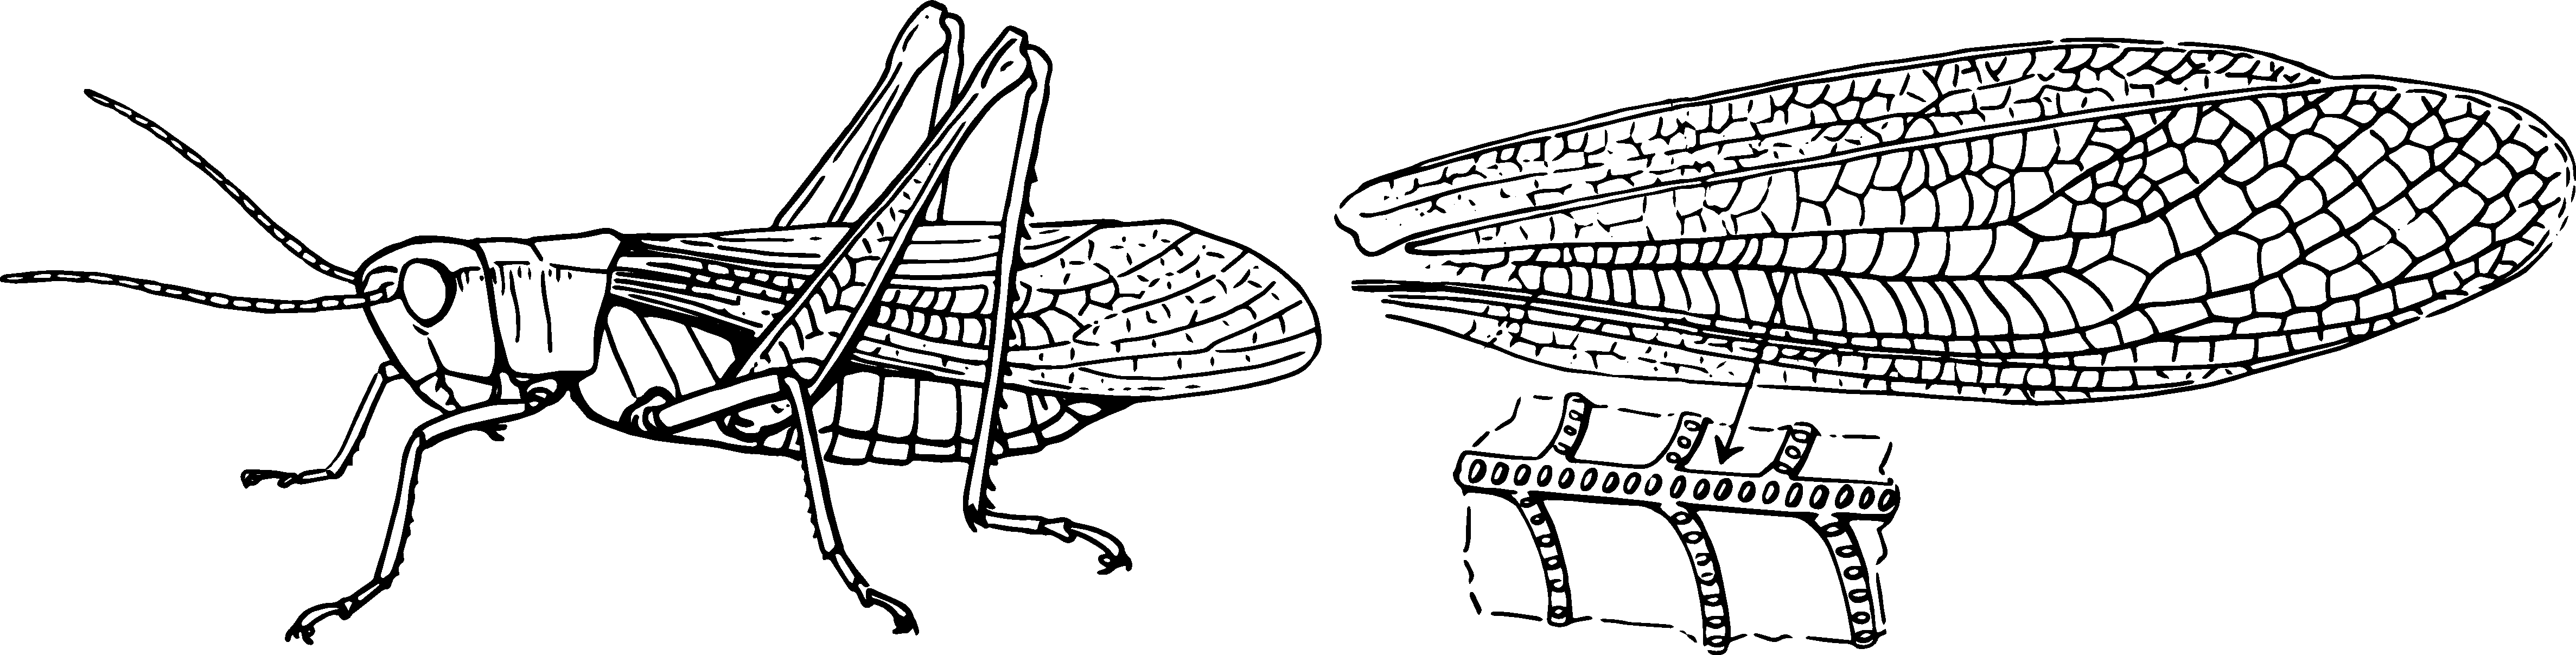
\includegraphics[width=0.92\textwidth]{polyneoptera/acrididae}}
  \caption{Acrididae \citep[modified from][Fig. 16]{bhl128276}}
  \label{fig:acrididhabitus}
\end{figure}

\subsection{Ensifera (crickets, katydids)}\index{Ensifera}
\begin{itemize}
\item antennae usually more than half as long as body, composed of more than 30 antennal sclerites
\item tarsi with 3--4 tarsomeres
\item auditory organ is usually present on the fore leg; can you locate this organ and compare with the auditory organ of Caelifera?
\item ovipositor long
\end{itemize}

\subsubsection{Tettigoniidae (long-horned grasshoppers, katydids)}\index{Tettigoniidae}
\noindent{}\textit{Diagnostic characters:} Tarsus with 4 tarsomeres; antennal foramina widely separated from each other; fore wing held roof-like over abdomen; ovipositor sword-shaped, usually curved; hind tibia with equally-sized spines; auditory organs present on front tibiae.\vspace{3mm}

\noindent{}\textit{Natural history:} Another large family, with more than 6,000 described species. Many of these insects are herbivores, but, unlike most orthopterans, many are predators.\vspace{3mm}

\begin{figure}[ht!]
    \centering
    \begin{subfigure}[ht!]{0.6\textwidth}
        \reflectbox{%
         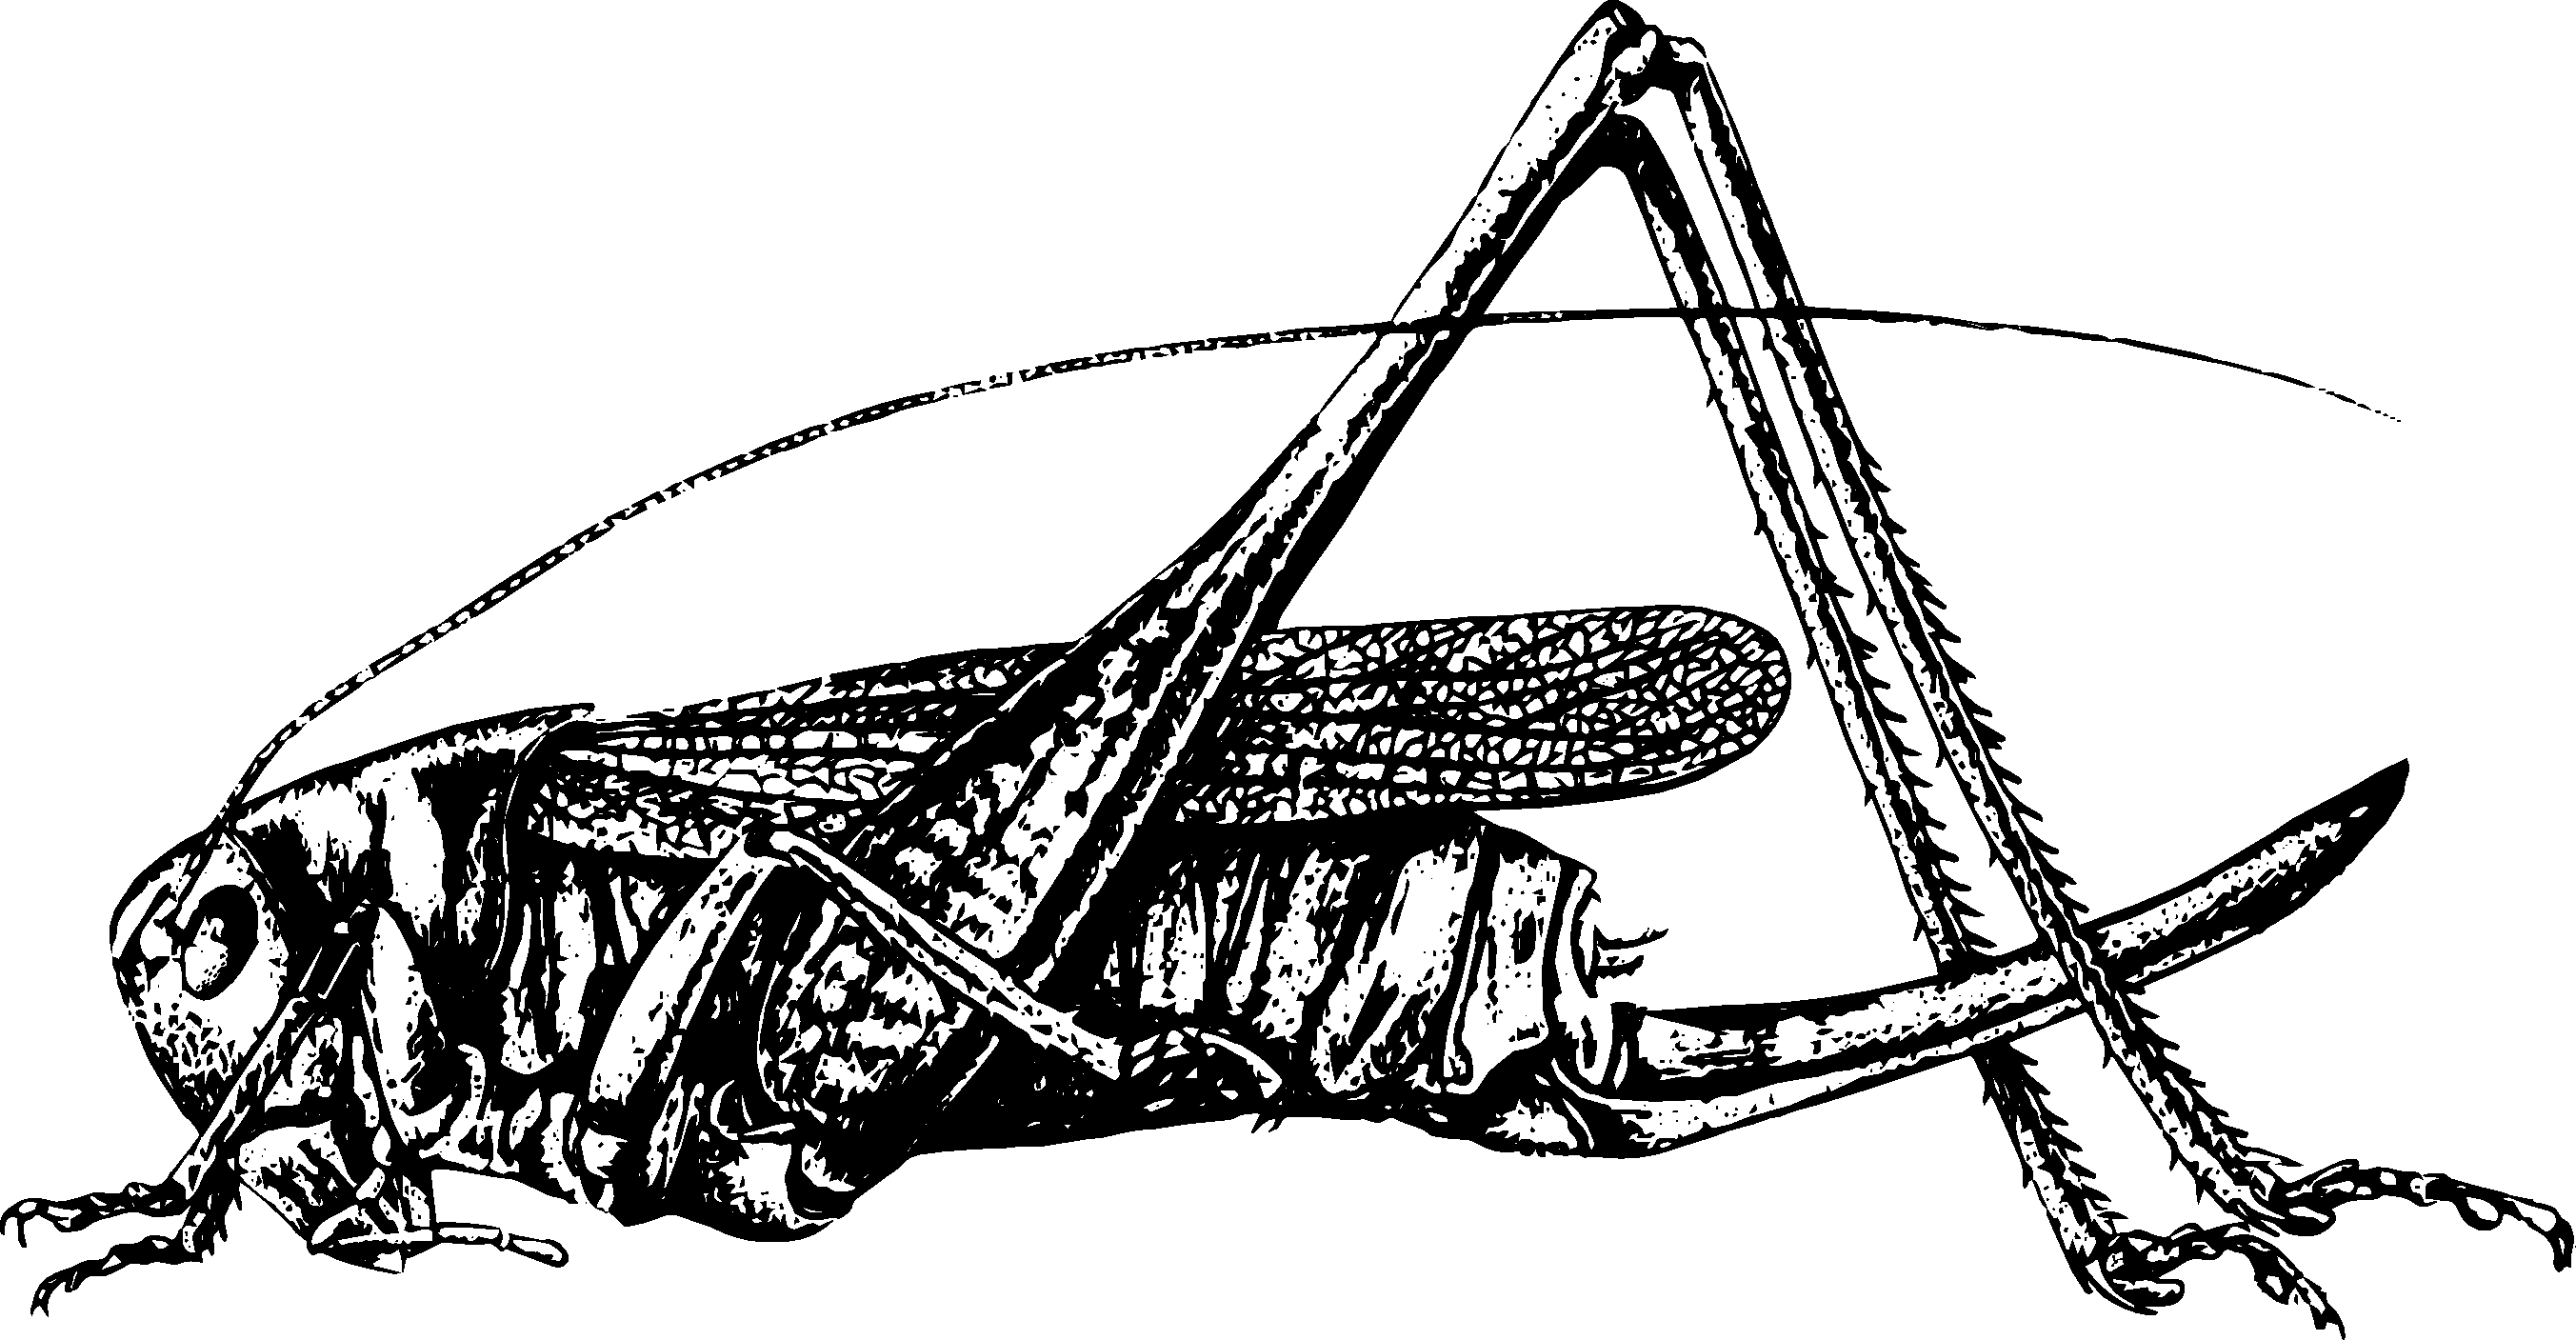
\includegraphics[width=\textwidth]{polyneoptera/tettigoniidae}}
        \caption{}
        \label{fig:tettihabitus}
    \end{subfigure}
    \qquad
    \begin{subfigure}[ht!]{0.09\textwidth}
        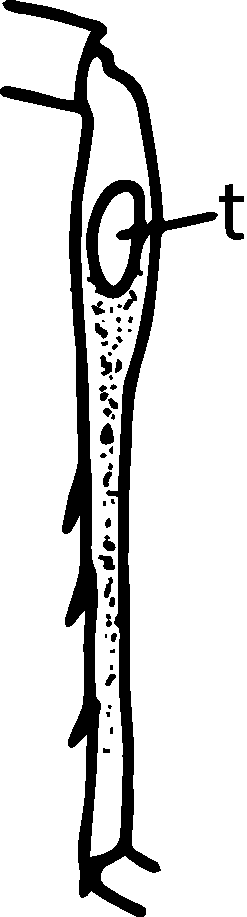
\includegraphics[width=\textwidth]{polyneoptera/tettiLeg}
        \caption{}
        \label{fig:tettiLeg}
    \end{subfigure}
    \caption{Tettigoniidae. \textbf{(a)} Habitus; \textbf{(b)} fore leg tibia, with tympanum (t) \citep[modified from][Figs. 20, 15A]{bhlitem15767}}\label{fig:tetti}
\end{figure}

\begin{theo}
{}Katydids have their ears in a very different part of their bodies, compared to grasshoppers. Do they also make sounds in different ways? Are these ears adapted for listening to other kinds of sounds?
\end{theo}

\subsubsection{Rhaphidophoridae (camel crickets)}\index{Rhaphidophoridae}
\noindent{}\textit{Diagnostic characters:} Mid tarsus subdivided into 4 tarsomeres, others 4 or 3; antennal foramina contiguous; wingless, usually humpbacked in appearance; ovipositor sword-shaped, usually curved; hind tibia with equally sized spines; auditory organ on fore tibia usually absent.\vspace{3mm}

\begin{theo}
{}Can you locate the pseudotympanum? Why is it called ``\textit{pseudo}tympanum''? What do all true tympana have in common structurally?
\end{theo}

\noindent{}\textit{Natural history:} Approximately 150 species can be found in North America, and all are associated with damp habitats (including caves, basements, sheds, wood piles). Some southwestern species live in deserts but are primarily active at night.\vspace{3mm}

\begin{figure}[ht!]
  \centering
    \reflectbox{
     \includegraphics[width=0.7\textwidth]{polyneoptera/raphido}}
  \caption{Rhaphidophoridae \citep[modified from][Fig. 25]{bhlitem15767}}
  \label{fig:rhaphid}
\end{figure}

\subsubsection{Grylloidea (crickets, trigs, tree crickets)}\index{Gryllidae}\index{Trigonidiidae}\index{Oecanthidae}\index{Grylloidea}\index{Mogoplistidae}
\noindent{}\textit{Diagnostic characters:} This taxon includes several families (e.g., Mogoplistidae, Oecanthidae, Trigonidiidae) that used to be classified within Gryllidae \citep{orthspecfile}. Tarsi subdivided into 3 tarsomeres; antennal foramina widely separated from each other; wings flattened on back, not roof-like; male fore wing often with veins and cells arranged in such a way that the pattern resembles a harp; ovipositor cylindrical, not usually curved; auditory organ present on fore tibia.\vspace{3mm}

\noindent{}\textit{Natural history:} Just under 1,000 species have been described worldwide, and many have impacted human culture through their singing and fighting habits. Most species are saprophages and opportunists.\vspace{3mm}

\noindent{}\textit{Specimen preparations:} Although they are pterygotes, adult crickets are best preserved in ethanol.\vspace{3mm}\index[preps]{Grylloidea}
\begin{figure}[ht!]
  \centering
    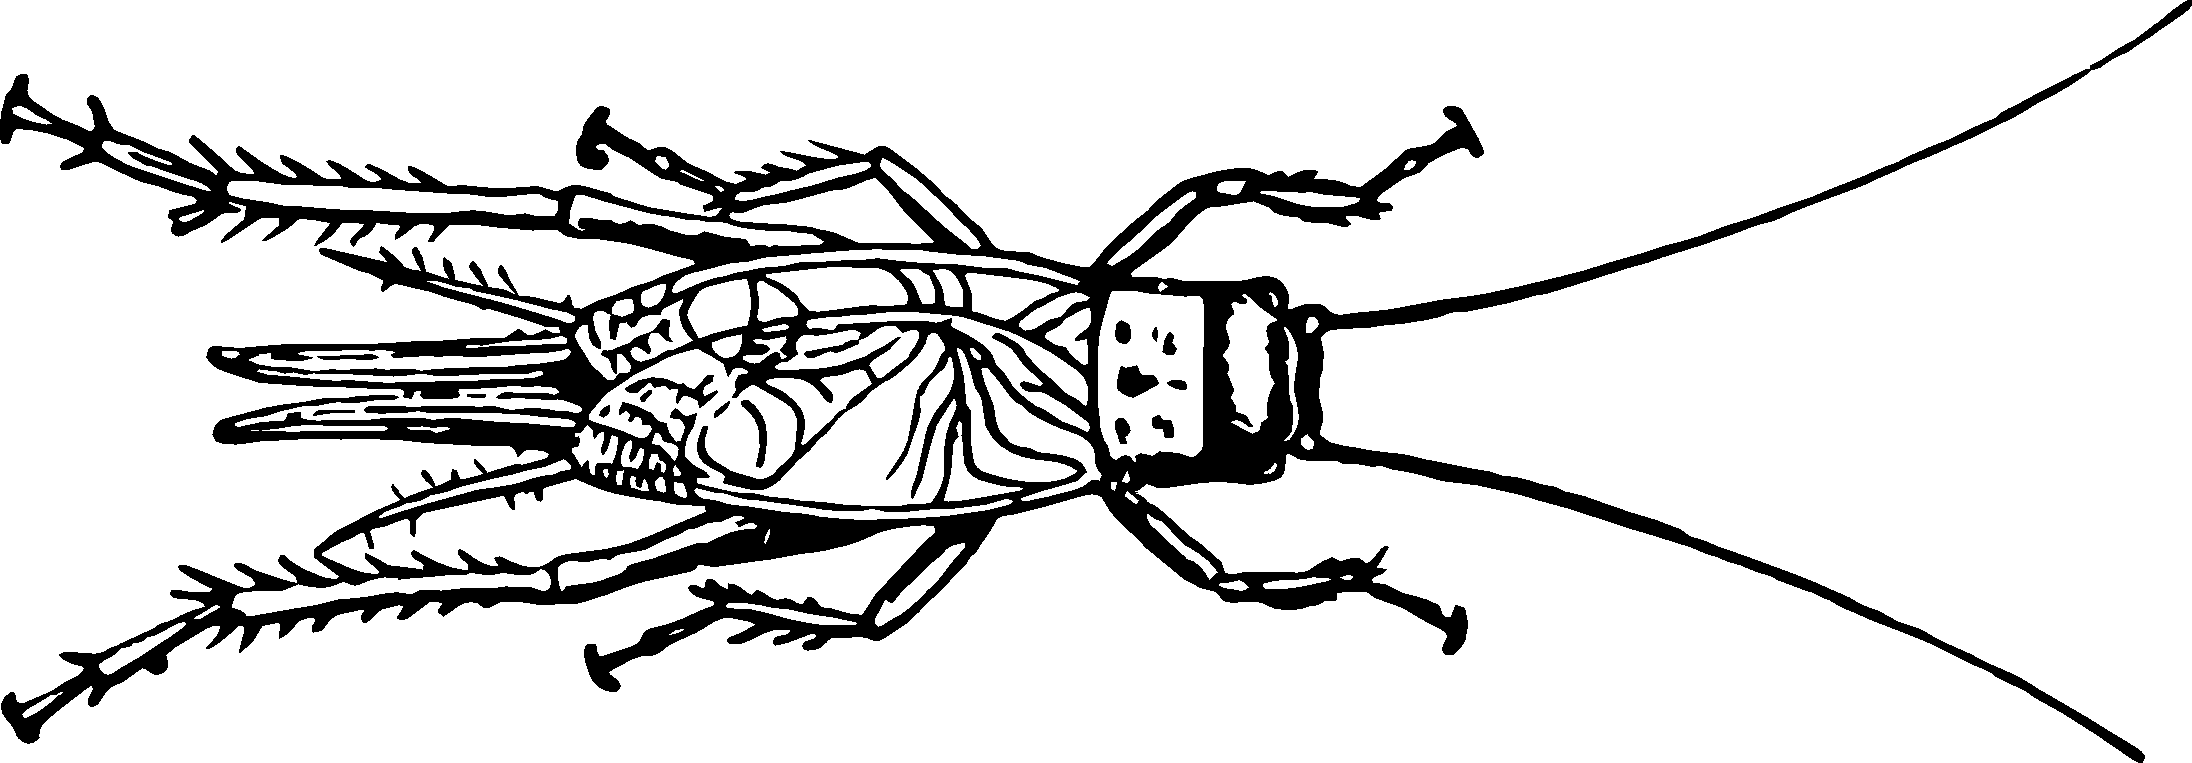
\includegraphics[width=0.6\textwidth]{polyneoptera/gryllid1}
  \caption{Gryllidae male \citep[modified from][Fig. 442]{leunis1877synopsis}}
  \label{fig:gryllidMale}
\end{figure}

\begin{figure}[ht!]
  \centering
    \includegraphics[width=0.6\textwidth]{polyneoptera/gryllid2}
  \caption{Gryllidae female \citep[modified from][Fig. 221]{kellogg1906american}}
  \label{fig:gryllid}
\end{figure}

\subsubsection{Gryllotalpidae (mole crickets)}\index{Gryllotalpidae}
\noindent{}\textit{Diagnostic characters:} Tarsi subdivided into 3 tarsomeres; antennal foramina widely separated from each other; wings flattened on back, not roof-like; male fore wing with ``harp''; fore leg fossorial; ovipositor short; hind tibia with alternating sized spines; auditory organ on fore tibia usually present; pseudotympanum on abdomen present.\vspace{3mm}

\noindent{}\textit{Natural history:} These insects burrow extensively in soil and can be pestiferous. They eat everything from vegetation to other invertebrates.\vspace{3mm}

\begin{figure}[ht!]
  \centering
    \includegraphics[width=0.7\textwidth]{polyneoptera/gryllotalpid}
  \caption{Gryllotalpidae \citep[modified from][Plate VII, Fig. 2]{bhlitem82061AustrInsect}}
  \label{fig:gryllotalp}
\end{figure}

\section{Dictyoptera}\index{Dictyoptera}
This lineage is sometimes treated as comprising three orders, especially in the older literature: Blattaria or Blattodea (cockroaches), Isoptera (termites), and Mantodea (mantids). Recent phylogenetic work strongly suggests that termites are derived cockroaches, \textit{i.e.}, that ``Blattaria'' is paraphyletic. Cockroaches and termites are referred to collectively as Blattodea. These insects can be recognized by the following characters: fore wings (if present) tegmen-like, with many crossveins; male genitalia asymmetrical (reduced in termites); ovipositor extremely reduced, mostly internal; eggs deposited in proteinaceous matrix or envelope (ootheca) formed from excretions of the accessory glands (apparently lost in most termites).

\subsection{Blattodea}\index{Blattodea}
\subsubsection{Blattidae (American cockroach, \textit{etc}.)}\index{Blattidae}
\noindent{}\textit{Diagnostic characters:} Fore wing (tegmen) more sclerotized than hind wing; female subgenital plate divided longitudinally; male styli similar to each other: slender, straight, elongate; spines on fore femur equal in length.\vspace{3mm}

\noindent{}\textit{Natural history:} This family is subdivided into 46 genera, including two commonly found in/around buildings (peridomestic): \textit{Periplaneta} and \textit{Blatta}. These insects deposit their oothecae after they're made, often burying them. \vspace{3mm}

\begin{figure}[ht!]
  \centering
    \includegraphics[width=0.6\textwidth]{polyneoptera/BlattidHabitus}
  \caption{Blattidae, dorsal and ventral habitus \citep[][Fig. 1]{bhl129194}}
  \label{fig:blattid1}
\end{figure}

\subsubsection{Ectobiidae (``Blattellidae''; German cockroach, \textit{etc}.)}\index{Ectobiidae}
\noindent{}\textit{Diagnostic characters:} Female subgenital plate not divided; male styli usually small, asymmetrical; spines on fore femur decrease in size apically.\vspace{3mm}

\noindent{}\textit{Natural history:} This family is subdivided into \textgreater200 genera, including many commonly found in/around buildings: \textit{e.g.}, \textit{Blattella} and \textit{Supella}. These insects often deposit their oothecae after they're made. Some species, however, hold onto them externally or even internally. This family is probably not monophyletic.\vspace{3mm}

\begin{figure}[ht!]
    \centering
    \begin{subfigure}[ht!]{0.45\textwidth}
        \includegraphics[width=\textwidth]{polyneoptera/EctobiidHabitus}
        \caption{}
        \label{fig:ectobiidhabitus}
    \end{subfigure}
    \qquad
    \begin{subfigure}[ht!]{0.45\textwidth}
        \includegraphics[width=\textwidth]{polyneoptera/EctobiidAbdomen}
        \caption{}
        \label{fig:ectobiidgenit}
    \end{subfigure}
    \caption{Ectobiidae. \textbf{(a)} Habitus, dorsal \citep[][Plate III, Fig. 14A]{bhl26431}; \textbf{(b)} ventral view of abdomen apex; male (l), female (r) \citep[Plate II, Fig. 7E,D]{bhl26431}}\label{fig:ectobiidae}
\end{figure}

\begin{theo}
{}Many insects are capable of walking or running quickly and efficiently. Why do you think cockroaches serve as the primary model for hexapodous robots? Is there something special about their morphology?
\end{theo}

\subsubsection{Cryptocercidae (hooded cockroaches)}\index{Cryptocercidae}
\noindent{}\textit{Diagnostic characters:} Apex of abdomen covered by 7th tergite dorsally, 6th sternite ventrally; no subgenital plate; always wingless; middle and hind femora with few spines relative to other families.\vspace{3mm}

\noindent{}\textit{Natural history:} These cockroaches are quite termite-like, with respect to their diet and interactions with conspecific individuals. In fact, Cryptocercidae is robustly sister to Isoptera. These cockroaches are described as being subsocial, with a common habitat (inside rotting wood) and considerable parental care of young.\vspace{3mm}

\begin{figure}[ht!]
  \centering
    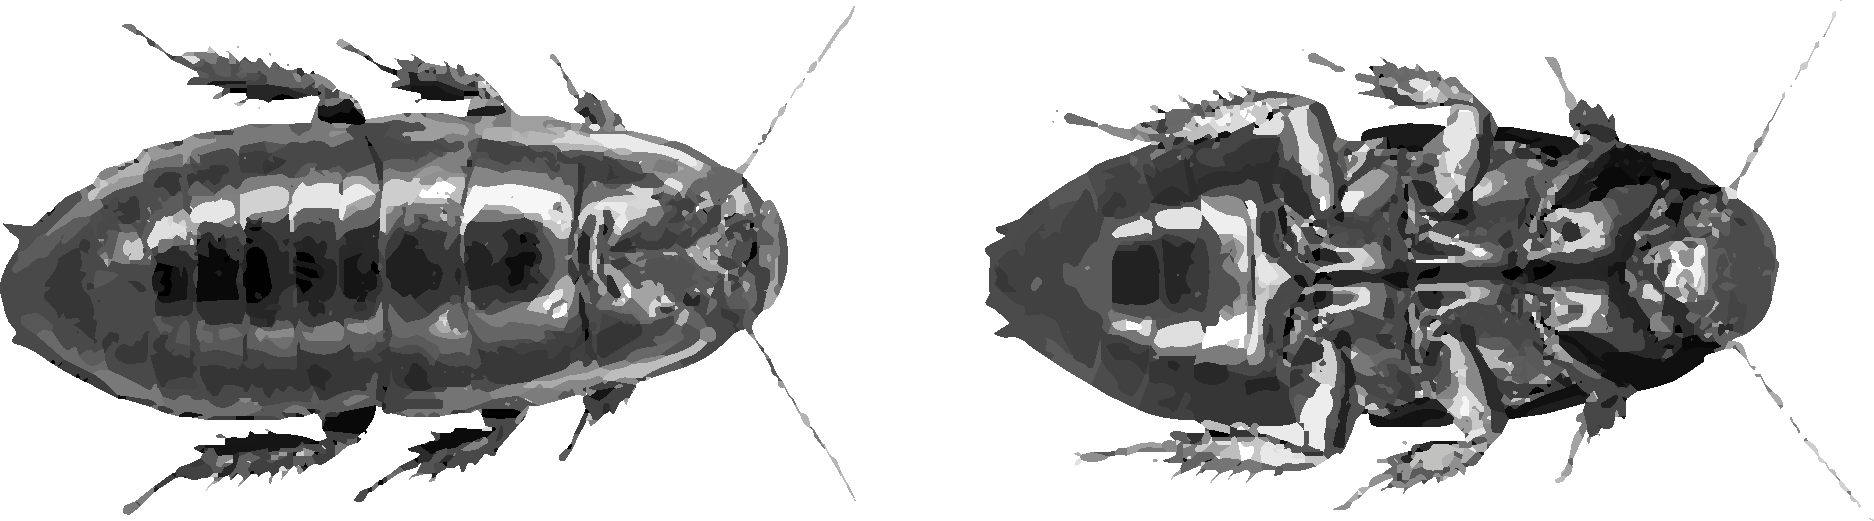
\includegraphics[width=0.7\textwidth]{sections/img/polyneoptera/cryptocercids.pdf}
  \caption{Cryptocercidae dorsal habitus \citep[modified from][Fig. 4f1,f2]{BaiCryptocercid}}
  \label{fig:cryptocercid}
\end{figure}

\subsubsection{Isoptera (termites)}\index{Isoptera}
\noindent{}\textit{Diagnostic characters:} Pronotum not shield-like (Compare to other Blattodea!); each tarsus subdivided into 4 tarsomeres (this character is difficult to see on dried specimens); cercus composed of 1--6 sclerites.\vspace{3mm}

\noindent{}\textit{Natural history:} The presence of a fontanelle (pore) on the head is used to diagnose families, as is the number of sclerotized wing veins along anterior margin of fore wing (\textit{e.g.}, two or three present). Can you find these features in our specimens? For soldiers, can you count the number of teeth on the inner margin of the left mandible? All species are eusocial and live in colonies. Their primary food source is wood. The 3,000 or so described species are primarily tropical.\vspace{3mm}

\begin{figure}[ht!]
  \centering
    \includegraphics[width=0.7\textwidth]{polyneoptera/Isoptera}
  \caption{Isoptera, alates, worker, soldier \citep[modified from][Plate II]{bhlitem82061AustrInsect}}
  \label{fig:termite}
\end{figure}

\subsection{Mantodea}\index{Mantodea}
\noindent{}\textit{Diagnostic characters:} Head roughly triangular, articulated with thorax via narrow neck (head highly mobile); face with area (facial or frontal shield) delimited by carinae; prothorax elongate, with raptorial fore legs; fore wings (if present) = tegmina; male genitalia asymmetrical.\vspace{3mm}

\noindent{}\textit{Natural history:} All $\sim$2,400 species are predators, and the bulk of their diversity lies in the tropics. A tympanum, located between their legs, on the sternum, is hypothesized to be an adaptation for bat avoidance.\vspace{3mm}

\noindent{}\textit{Specimen preparations:} \cite{mantidPreservation} provide detailed best practices regarding how to preserve Mantodea, with fore legs and right wings spread.\vspace{3mm}\index[preps]{Mantodea}

\begin{figure}[ht!]
  \centering
    \reflectbox{
     \includegraphics[width=0.7\textwidth]{polyneoptera/mantis}}
  \caption{Mantodea \citep[modified from][plate 78]{bhlitem122043}}
  \label{fig:mantidbody}
\end{figure}

\begin{figure}[ht!]
    \centering
    \begin{subfigure}[ht!]{0.35\textwidth}
        \includegraphics[width=\textwidth]{polyneoptera/MantodeaHead}
        \caption{}
        \label{fig:mantodea1}
    \end{subfigure}
    \qquad
    \begin{subfigure}[ht!]{0.45\textwidth}
        \includegraphics[width=\textwidth]{polyneoptera/MantodeaForeLeg}
        \caption{}
        \label{fig:mantodea2}
    \end{subfigure}
    \caption{Mantodea. \textbf{(a)} Head, anterior view \citep[modified from][Plate 130, Fig. 1a]{bhl24070}; \textbf{(b)} raptorial fore leg \citep[modified from][Plate 130, Fig. 1f]{bhl24070}}\label{fig:mantodeans}
\end{figure}

\section{Grylloblattodea (ice crawlers)}\index{Grylloblattodea}
\subsubsection{Grylloblattidae}
\noindent{}\textit{Diagnostic characters:} Head prognathous; compound eyes reduced or absent; wings absent; cerci multi-segmented.\vspace{3mm}

\noindent{}\textit{Natural history:} These insects are cryophilic and can only be found---at least in North America---associated with high elevations and snow pack. They are thought to be predators or scavengers of dead insects, but they will also eat plant material. There are about 30 species known worldwide.\vspace{3mm}

\begin{figure}[ht!]
  \centering
    \includegraphics[width=0.55\textwidth]{polyneoptera/Grylloblatta}
  \caption{Grylloblattodea \citep[modified from][Figs. 1--2]{walker1914new}}
  \label{fig:grylloblatt}
\end{figure}

\section{Mantophasmatodea (heel-walkers, gladiators)}\index{Mantophasmatodea}

\noindent{}\textit{Diagnostic characters:} Head hypognathous; antennae long, with spindle-shaped flagellomeres distally; arolium (pad-like structure on the distal end of each leg) expanded, held aloft when moving; legs adapted for grabbing prey (spiny); wingless.\vspace{3mm}

\noindent{}\textit{Natural history:} These insects are all predators. Extant species can only be found in southern Africa.\vspace{3mm}

\begin{theo}
{}Although they are relatively common, heel-walkers were only discovered recently (2001). Why did researchers overlook members of this taxon for so long?
\end{theo} \vspace{3mm}

\begin{figure}[ht!]
  \centering
    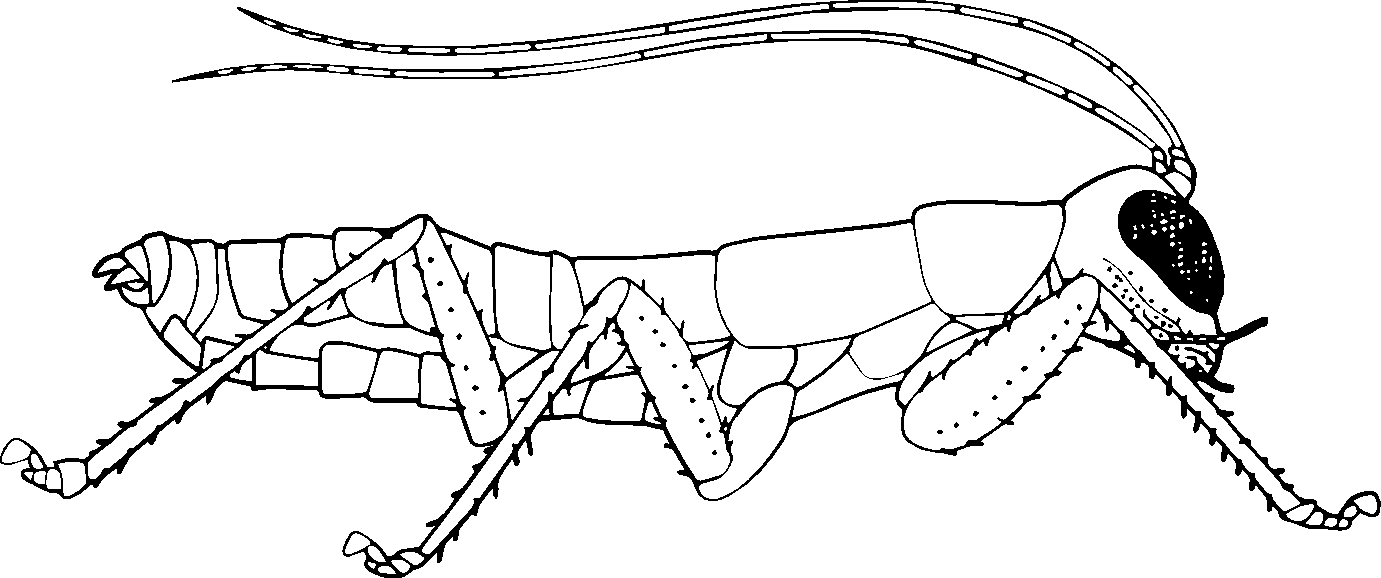
\includegraphics[width=0.6\textwidth]{polyneoptera/mantophasmatodea4}
  \caption{Mantophasmatodea (illustration by Laura Porturas)}
  \label{fig:mantophas}
\end{figure}

\section{Embioptera (webspinners, Embiodea, Embiidina)}\index{Embioptera}
\noindent{}\textit{Diagnostic characters:} Body nearly cylindrical; head prognathous; proximalmost tarsomere greatly expanded to accommodate silk-producing glands;  wings (males only) highly flexible, similar in size/shape; male genitalia asymmetrical.\vspace{3mm}

\noindent{}\textit{Natural history:} Only a handful of species occur in the U.S., and none (yet) can be found in the northeastern states. Males, which are rarely collected in the eastern U.S., are typically needed for family-level identification. These insects live communally in silken galleries, usually under rocks and logs and on tree trunks.\vspace{3mm}

\begin{figure}[ht!]
    \centering
    \begin{subfigure}[b!]{0.45\textwidth}
        \includegraphics[width=\textwidth]{polyneoptera/EmbiopteraF}
        \caption{}
        \label{fig:embiop1}
    \end{subfigure}
    \qquad
    \begin{subfigure}[ht!]{0.4\textwidth}
        \includegraphics[width=\textwidth]{polyneoptera/EmbiopteraM}
        \caption{}
        \label{fig:embiop2}
    \end{subfigure}
    \caption{Embioptera. \textbf{(a)} Female \citep[modified from][Plate 1, Fig. D]{bhl37580}; \textbf{(b)} male \citep[modified from][Plate 130, Fig. C]{bhl37580}}\label{fig:embiops}
\end{figure}

\section{Phasmida (Phasmatodea; walking sticks, leaf insects)}\index{Phasmida}
\begin{itemize}
\item frons anterolaterally convex
\item prothroax with defensive gland openings
\item trochanter+femur nearly fused
\end{itemize}

\subsubsection{Diapheromeridae (common walkingsticks)}\index{Diapheromeridae}
\noindent{}\textit{Diagnostic characters:} Mesothorax at least 4$\times$ as long as prothorax; each leg with 5 tarsomeres; head without spines posteriorly; 1st abdominal segment shorter than metathorax; usually wingless.\vspace{3mm}

\noindent{}\textit{Natural history:} Only two species occur in the U.S., and both of them, like all walking sticks, eat vegetation.

\begin{figure}[ht!]
  \centering
    \includegraphics[width=0.7\textwidth]{polyneoptera/heteronemiid}
  \caption{Diapheromeridae \citep[modified from][Fig. 118]{bhlitem16801}}
  \label{fig:heteronemiid}
\end{figure}

\section*{Test yourself}
We talked about several adaptations to protect eggs from desiccation and predation, especially (but not exclusively!) in Dictyoptera. Can you describe them?\vspace{3mm}

\noindent{}What evidence do we have to suggest that termites are derived cockroaches? Describe three aspects of their natural history that may have led to the evolution of eusociality.\vspace{3mm}

\noindent{}Why do some taxa---\textit{e.g.}, Embioptera and Zoraptera---live communally?

\clearpage
\thispagestyle{empty}